\section{Carbon Intensity Analysis}
The data distribution goes from 2021-01 to 2024-01. \\
In this case data hasn’t been manipulated in any way, as no interpolation has been applied. \\
With carbon intensity is much easier to highlight patterns and trends; in this case we are considering the carbon intensity related to direct power and energy usage, specific for our country (Italy) and area (Emilia-Romagna).

\vspace{-15pt}

\begin{figure}[H]
\centering
\includegraphics[width=1\textwidth]{../../PLOTS/CI_direct.png}
\captionsetup{skip=-10pt}
\caption{CI direct}
\label{fig:CI_direct}
\end{figure}

\vspace{-20pt}

\begin{figure}[H]
\centering
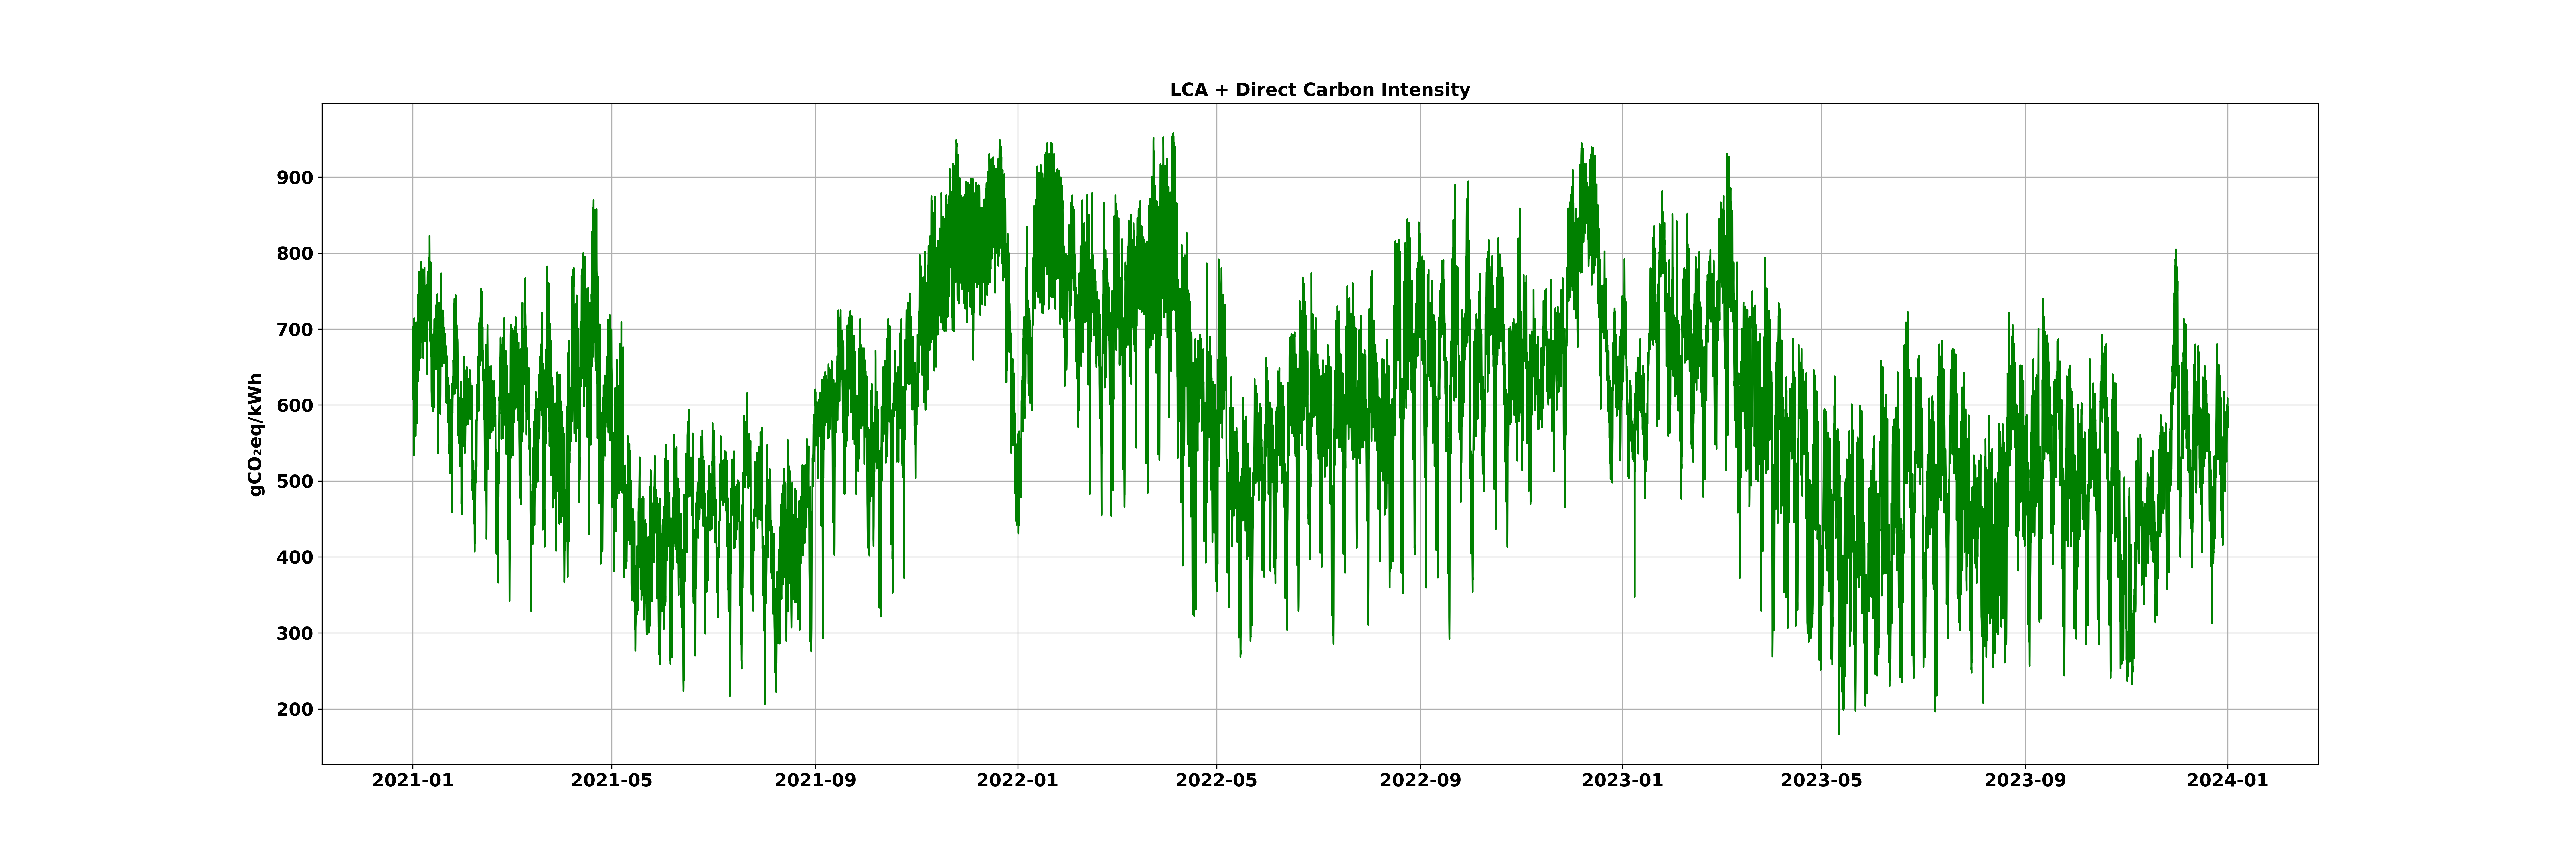
\includegraphics[width=1\textwidth]{../../PLOTS/CI_LCA+direct.png}
\captionsetup{skip=-10pt}
\caption{CI LCA + direct}
\label{CI_LCA+direct}
\end{figure}

\begin{center}
\setstretch{0.9}
count    26280.000000 \\
mean       258.794563 \\
std         63.450587 \\
min         67.790000 \\
25\%        214.945000 \\
50\%        260.075000 \\
75\%        302.832500 \\
max        424.440000
\end{center}

\subsection{CI comparison}
Both direct and indirect (LCA) carbon intensity share a similar pattern, showing equal highs and lows in time. Also the sum of the two distributions has the same behaviour.  

\vspace{-15pt}

\begin{figure}[H]
\centering
\includegraphics[width=1\textwidth]{../../PLOTS/CI_comparison.png}
\captionsetup{skip=-10pt}
\caption{CI comparison}
\label{CI_comparison}
\end{figure}

\subsection{CI STL}
Taking advantage of this decomposition we can easily guess the following assumptions: carbon intensity has a strong seasonality, showing a visible decrease during the warmer months and the opposite during cold ones; in addition there seems to be a strong decrease in the CI every January.

\vspace{-15pt}

\begin{figure}[H]
\centering
\includegraphics[width=1\textwidth]{../../PLOTS/CI_stl.png}
%\captionsetup{skip=-10pt}
\caption{CI STL}
\label{CI_stl}
\end{figure}

\subsection{CI analysis using Meta's Prophet}
At deeper level (daily, weekly or monthly), much clearer patterns are visible: \\
During week days the carbon intensity is higher with respect to weekends, as well as the CI contribution decreases during the lunch time (noon). Finally we can better visualise what we guessed before: during the year we see a couple of peaks, near February and December, with a lowering during January, contrary to what happens from May to September, where the general CI contribution goes down.

\vspace{-15pt}

\begin{figure}[H]
\centering
\includegraphics[width=1\textwidth]{../../PLOTS/CI_prophet.png}
%\captionsetup{skip=-10pt}
\caption{CI trends}
\label{CI_prophet}
\end{figure}